% ============================================================
% CAPÍTULO 33: CAMPOS VECTORIALES E INTEGRALES DE LÍNEA
% ============================================================

\chapter{Campos vectoriales e integrales de línea}

En este módulo se estudian los \textbf{campos vectoriales} —funciones que
asignan un vector a cada punto del espacio— y en particular los
\textbf{campos conservativos}, que son aquellos que provienen del
gradiente de una función escalar. Estos campos gozan de una propiedad
notable: el trabajo realizado a lo largo de una trayectoria no depende
del camino recorrido, sino únicamente de los puntos inicial y final.

En segundo lugar, se introduce la \textbf{integral de línea de un campo
escalar}, una herramienta que generaliza la integral definida a
trayectorias curvas en el plano o en el espacio. Esta integral permite
acumular cantidades como masa, carga o temperatura a lo largo de un
camino, y su cálculo se reduce a una integral ordinaria mediante una
parametrización adecuada de la curva.

Ambos conceptos son pilares del cálculo multivariable y tienen
aplicaciones directas en física, ingeniería y geometría. La conexión
entre ellos aparece cuando el campo escalar es una función potencial:
entonces la integral de línea del campo vectorial gradiente se evalúa
simplemente como la diferencia de potencial entre los extremos.

\section{Campos Vectoriales}

\begin{definition}[Campo vectorial]
Un \textbf{campo vectorial} en \(\mathbb{R}^3\) es una función
\(\mathbf{F}: D \subseteq \mathbb{R}^3 \to \mathbb{R}^3\) que asigna a
cada punto \((x,y,z)\) de su dominio un vector tridimensional. Se
escribe como
\[
\mathbf{F}(x,y,z) = M(x,y,z)\,\mathbf{i} + N(x,y,z)\,\mathbf{j}
+ P(x,y,z)\,\mathbf{k},
\]
donde \(M,N,P\) son funciones escalares llamadas \textbf{componentes}
del campo. En \(\mathbb{R}^2\), un campo vectorial tiene la forma
\[
\mathbf{F}(x,y) = M(x,y)\,\mathbf{i} + N(x,y)\,\mathbf{j}.
\]
\end{definition}
\begin{rem}
Los campos vectoriales modelan magnitudes que tienen dirección y
sentido en cada punto del espacio. Ejemplos físicos incluyen:
\begin{itemize}
  \item el campo de velocidades de un fluido (cada partícula se mueve
  con la velocidad indicada por el campo),
  \item el campo gravitacional (la fuerza que experimenta una masa
  unitaria),
  \item el campo eléctrico (la fuerza por unidad de carga),
  \item el campo magnético.
\end{itemize}
\end{rem}

\begin{definition}[Continuidad y diferenciabilidad de un campo vectorial]
Un campo vectorial \(\mathbf{F} = M\mathbf{i}+N\mathbf{j}+P\mathbf{k}\)
es \textbf{continuo} en una región \(D\) si cada una de sus funciones
componentes \(M,N,P\) es continua en \(D\). Es \textbf{diferenciable}
si cada componente tiene derivadas parciales continuas en \(D\).
\end{definition}

\begin{definition}[Campo vectorial gradiente]
Dada una función escalar \(f: D \subseteq \mathbb{R}^n \to \mathbb{R}\)
diferenciable, su \textbf{gradiente} es el campo vectorial definido por
\[
\nabla f(x,y) = f_x(x,y)\,\mathbf{i} + f_y(x,y)\,\mathbf{j}
\quad \text{en } \mathbb{R}^2,
\]
y
\[
\nabla f(x,y,z) = f_x(x,y,z)\,\mathbf{i}
+ f_y(x,y,z)\,\mathbf{j}
+ f_z(x,y,z)\,\mathbf{k}
\quad \text{en } \mathbb{R}^3.
\]
\end{definition}

\begin{figure}[H]
\centering
\begin{tikzpicture}[scale=1.05]
  % Ejes
  \draw[->,thin] (-2.4,0)--(2.4,0) node[anchor=west] {$x$};
  \draw[->,thin] (0,-2.3)--(0,2.4) node[anchor=south] {$y$};
  % Curvas de nivel f(x,y)=x^2+y^2/4  (elipses: semi-eje x=sqrt(c), y=2*sqrt(c))
  % c=0.25: a=0.50, b=1.00
  \draw[blue!70,thick] (0,0) ellipse (0.50 and 1.00);
  \node[blue,font=\scriptsize,anchor=north west] at (0.52,0.02) {$\tfrac{1}{4}$};
  % c=0.50: a=0.707, b=1.414
  \draw[blue!70,thick] (0,0) ellipse (0.71 and 1.41);
  \node[blue,font=\scriptsize,anchor=north west] at (0.73,0.02) {$\tfrac{1}{2}$};
  % c=1.00: a=1.00, b=2.00
  \draw[blue!70,thick] (0,0) ellipse (1.00 and 2.00);
  \node[blue,font=\scriptsize,anchor=north west] at (1.02,0.02) {$1$};
  % Vectores gradiente nabla f = (2x, y/2); escala k=0.14
  \foreach \xi/\yi in {
      -1.6/-1.6, -1.6/-0.8, -1.6/0.8, -1.6/1.6,
      -0.8/-1.6, -0.8/-0.8, -0.8/0.8, -0.8/1.6,
       0.8/-1.6,  0.8/-0.8,  0.8/0.8,  0.8/1.6,
       1.6/-1.6,  1.6/-0.8,  1.6/0.8,  1.6/1.6} {
    \pgfmathsetmacro\dx{2*\xi*0.14}
    \pgfmathsetmacro\dy{\yi/2*0.14}
    \draw[->,red!70!black,thin] (\xi,\yi)--++(\dx,\dy);
  }
  % Leyendas
  \node[red!70!black,anchor=north east,font=\small] at (2.3,-2.1)
    {$\nabla f=(2x,\tfrac{y}{2})$};
  \node[blue!80!black,anchor=south east,font=\small] at (2.3,0.1)
    {$f(x,y)=x^2+\tfrac{y^2}{4}$};
\end{tikzpicture}
\caption{Campo gradiente $\nabla f=(2x,\,\tfrac{y}{2})$ (flechas rojas) perpendicular
  a las curvas de nivel $f(x,y)=c$ (elipses azules) de $f(x,y)=x^2+\tfrac{y^2}{4}$}
\label{fig:campo_gradiente}
\end{figure}
\begin{rem}[Interpretación geométrica del gradiente]
El vector \(\nabla f(P)\) apunta en la dirección de \textbf{máximo
crecimiento} de \(f\) en el punto \(P\), y su norma
\(\|\nabla f(P)\|\) mide la tasa de cambio de \(f\) en esa dirección.
Además, \(\nabla f(P)\) es perpendicular a las curvas (o superficies)
de nivel de \(f\) que pasan por \(P\).
\end{rem}

\begin{definition}[Campo vectorial conservativo]
Un campo vectorial \(\mathbf{F}\) se dice \textbf{conservativo} si
existe una función escalar \(\Phi\), llamada \textbf{función
potencial}, tal que
\[
\mathbf{F} = \nabla \Phi.
\]
Es decir, un campo conservativo es el gradiente de alguna función
escalar. En este caso, el campo se denomina \textbf{campo gradiente}.
\end{definition}

\begin{figure}[H]
\centering
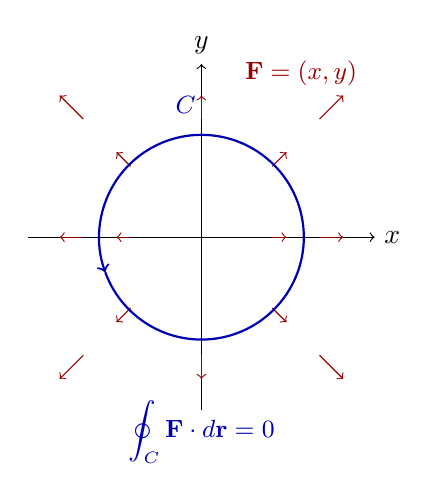
\begin{tikzpicture}[scale=1.0]
  % Ejes
  \draw[->,thin] (-2.2,0)--(2.2,0) node[anchor=west] {$x$};
  \draw[->,thin] (0,-2.2)--(0,2.2) node[anchor=south] {$y$};
  % Vectores del campo F=(x,y); escala k=0.20
  \foreach \xi/\yi in {
      -1.5/-1.5, -1.5/0, -1.5/1.5,
      -0.9/-0.9, -0.9/0, -0.9/0.9,
       0/-1.5, 0/1.5,
       0.9/-0.9, 0.9/0, 0.9/0.9,
       1.5/-1.5, 1.5/0, 1.5/1.5} {
    \pgfmathsetmacro\dx{\xi*0.20}
    \pgfmathsetmacro\dy{\yi*0.20}
    \draw[->,red!60!black,thin] (\xi,\yi)--++(\dx,\dy);
  }
  % Curva cerrada (círculo de radio 1.3, con orientación)
  \draw[blue!70!black,thick,->] (1.3,0) arc(0:200:1.3);
  \draw[blue!70!black,thick]    (1.3,0) arc(0:-160:1.3);
  \node[blue!70!black,anchor=south,font=\small] at (-0.2,1.45) {$C$};
  % Anotación integral cero
  \node[blue!70!black,anchor=north,font=\small] at (0,-1.95)
    {$\displaystyle\oint_C \mathbf{F}\cdot d\mathbf{r}=0$};
  % Leyenda campo
  \node[red!60!black,anchor=south east,font=\small] at (2.1,1.8)
    {$\mathbf{F}=(x,y)$};
\end{tikzpicture}
\caption{Campo conservativo $\mathbf{F}(x,y)=(x,y)=\nabla\!\left(\tfrac{x^2+y^2}{2}\right)$:
  las flechas apuntan radialmente; la integral sobre cualquier curva cerrada $C$ es cero}
\label{fig:campo_conservativo}
\end{figure}
\begin{theorem}[Caracterización de campos conservativos en el plano]
Sean \(M(x,y)\) y \(N(x,y)\) funciones con derivadas parciales continuas
en una región abierta \(R\). El campo vectorial
\(\mathbf{F}(x,y) = M(x,y)\mathbf{i} + N(x,y)\mathbf{j}\) es
conservativo si y solo si
\[
\frac{\partial N}{\partial x} = \frac{\partial M}{\partial y}
\quad \text{en } R.
\]
\end{theorem}

\begin{rem}
La condición \(\partial N/\partial x = \partial M/\partial y\) es
necesaria y suficiente para la existencia de función potencial en
regiones \emph{simplemente conexas} (es decir, sin agujeros). En
regiones con agujeros, la igualdad de derivadas cruzadas no basta:
puede haber campos con rotacional nulo que no sean conservativos.
\end{rem}

\begin{rem}[Propiedades de los campos conservativos]
Si \(\mathbf{F} = \nabla \Phi\) es conservativo, entonces:
\begin{enumerate}
  \item La integral de línea de \(\mathbf{F}\) entre dos puntos
  \emph{no depende del camino} seguido, sino solo de los puntos
  inicial y final.
  \item En regiones simplemente conexas, su rotacional es nulo:
  \[
  \nabla \times \mathbf{F} = \mathbf{0}.
  \]
  \item El trabajo realizado por \(\mathbf{F}\) a lo largo de una
  curva cerrada es cero.
\end{enumerate}
\end{rem}

\begin{example}[Verificación de campo conservativo en el plano]
Determine si el campo
\[
\mathbf{F}(x,y) = (2x y)\,\mathbf{i} + (x^2 + 3y^2)\,\mathbf{j}
\]
es conservativo. En caso afirmativo, halle su función potencial.
\begin{myproof}
\textbf{Paso 1. Identificar componentes.}
Aquí \(M(x,y) = 2xy\) y \(N(x,y) = x^2 + 3y^2\).

\textbf{Paso 2. Verificar condición de igualdad de derivadas cruzadas.}
Calculamos:
\[
\frac{\partial N}{\partial x} = 2x, \qquad
\frac{\partial M}{\partial y} = 2x.
\]
Como \(\partial N/\partial x = \partial M/\partial y\), el campo
cumple la condición necesaria en todo \(\mathbb{R}^2\), que es una
región simplemente conexa. Por tanto, \(\mathbf{F}\) es conservativo.

\textbf{Paso 3. Hallar la función potencial.}
Buscamos \(\Phi(x,y)\) tal que \(\nabla \Phi = \mathbf{F}\):
\[
\Phi_x = 2xy, \qquad \Phi_y = x^2 + 3y^2.
\]
Integramos \(\Phi_x\) respecto a \(x\):
\[
\Phi(x,y) = \int 2xy \, dx = x^2 y + g(y).
\]
Derivamos respecto a \(y\):
\[
\Phi_y = x^2 + g'(y).
\]
Igualamos con la segunda componente:
\[
x^2 + g'(y) = x^2 + 3y^2 \implies g'(y) = 3y^2.
\]
Integrando: \(g(y) = y^3 + C\). Por tanto:
\[
\Phi(x,y) = x^2 y + y^3 + C.
\]
Verificamos: \(\nabla \Phi = (2xy)\,\mathbf{i} + (x^2+3y^2)\,\mathbf{j} = \mathbf{F}\).

\textbf{Paso 4. Resultado.}
\[
\boxed{\mathbf{F} \text{ es conservativo con función potencial } \Phi(x,y) = x^2 y + y^3 + C.}
\]
\end{myproof}
\end{example}

\section{Integral de línea de un campo escalar}

La integral de línea de un campo escalar generaliza la integral definida a curvas. En lugar de integrar sobre un intervalo en el eje \(x\), se integra sobre una curva \(C\) en el plano o en el espacio, acumulando los valores de una función escalar \(f\) a lo largo de la
curva.

\begin{definition}[Integral de línea sobre un campo escalar]
Sea \(C\) una curva suave en \(\mathbb{R}^2\) parametrizada por
\(\mathbf{r}(t) = (x(t), y(t))\), con \(a \le t \le b\). Dividimos
el intervalo \([a,b]\) en \(n\) subintervalos, lo que induce una
partición de la curva en pequeños segmentos de longitud \(\Delta s_i\).
En cada segmento elegimos un punto \((x_i^*, y_i^*)\) y formamos la
suma
\[
\sum_{i=1}^n f(x_i^*, y_i^*) \,\Delta s_i.
\]
La \textbf{integral de línea de \(f\) a lo largo de \(C\)} es el
límite de estas sumas cuando la partición se refina:
\[
\int_C f(x,y)\,ds = \lim_{n\to\infty}
\sum_{i=1}^n f(x_i^*, y_i^*) \,\Delta s_i.
\]
En \(\mathbb{R}^3\), la definición es análoga:
\[
\int_C f(x,y,z)\,ds = \lim_{n\to\infty}
\sum_{i=1}^n f(x_i^*, y_i^*, z_i^*) \,\Delta s_i.
\]
\end{definition}
\begin{rem}
La notación \(ds\) representa el \textbf{elemento de longitud de
arco}. Para una curva parametrizada \(\mathbf{r}(t)\),
\[
ds = \|\mathbf{r}'(t)\|\,dt.
\]
Esta relación es la clave para evaluar la integral de línea mediante
una integral definida ordinaria.
\end{rem}

\begin{pasos}[Evaluación de una integral de línea de campo escalar]
Para calcular \(\int_C f\,ds\), se sigue este protocolo:
\begin{enumerate}
  \item \textbf{Parametrizar la curva.} Obtener una parametrización
  \(\mathbf{r}(t) = (x(t), y(t), z(t))\), \(a \le t \le b\), que
  recorra la curva \(C\).
  \item \textbf{Calcular la rapidez.} Hallar
  \(\|\mathbf{r}'(t)\| = \sqrt{(x')^2 + (y')^2 + (z')^2}\).
  \item \textbf{Sustituir en el integrando.} Reemplazar \(x,y,z\) por
  \(x(t),y(t),z(t)\) en \(f\).
  \item \textbf{Integrar.} Evaluar la integral definida
  \[
  \int_a^b f(x(t),y(t),z(t)) \,\|\mathbf{r}'(t)\|\,dt.
  \]
\end{enumerate}
\end{pasos}

\begin{theorem}[Teorema de evaluación para integral de línea de campo escalar]
Sea \(C\) una curva suave en \(\mathbb{R}^2\) parametrizada por
\(\mathbf{r}(t) = (x(t), y(t))\), \(a \le t \le b\), con \(x(t)\) y
\(y(t)\) derivables con derivadas continuas. Sea \(f\) continua en
una región que contiene a \(C\). Entonces
\[
\int_C f(x,y)\,ds =
\int_a^b f(x(t), y(t)) \sqrt{[x'(t)]^2 + [y'(t)]^2}\,dt.
\]
Análogamente, en \(\mathbb{R}^3\):
\[
\int_C f(x,y,z)\,ds =
\int_a^b f(x(t), y(t), z(t)) \sqrt{[x'(t)]^2 + [y'(t)]^2 + [z'(t)]^2}\,dt.
\]
\end{theorem}

\begin{rem}[Curvas suaves por partes]
Muchas curvas no son completamente suaves, pero pueden descomponerse en
un número finito de curvas suaves \(C_1, C_2, \dots, C_n\). En tal caso,
\[
\int_C f\,ds = \int_{C_1} f\,ds + \int_{C_2} f\,ds + \cdots + \int_{C_n} f\,ds.
\]
Esta propiedad es consecuencia directa de la aditividad de la integral
definida.
\end{rem}

\begin{rem}[Independencia de la orientación para campos escalares]
A diferencia de las integrales de línea de campos vectoriales, la
integral de línea de un campo escalar \emph{no} cambia de signo al
recorrer la curva en sentido contrario:
\[
\int_{-C} f\,ds = \int_C f\,ds.
\]
Esto se debe a que \(ds\) es siempre positivo, independientemente de
la orientación.
\end{rem}

\begin{example}[Integral de línea de un campo escalar en el plano]
Calcule \(\displaystyle \int_C (x + y)\,ds\), donde \(C\) es el
segmento de recta desde \((0,0)\) hasta \((1,2)\).
\begin{myproof}
\textbf{Paso 1. Parametrizar la curva.}
El segmento se parametriza como
\[
\mathbf{r}(t) = (1-t)(0,0) + t(1,2) = (t, 2t), \qquad 0 \le t \le 1.
\]

\textbf{Paso 2. Calcular la rapidez.}
\[
\mathbf{r}'(t) = (1, 2) \implies
\|\mathbf{r}'(t)\| = \sqrt{1^2 + 2^2} = \sqrt{5}.
\]

\textbf{Paso 3. Sustituir en el integrando.}
\(f(x,y) = x + y\), luego
\[
f(x(t), y(t)) = t + 2t = 3t.
\]

\textbf{Paso 4. Integrar.}
\[
\int_C (x+y)\,ds =
\int_0^1 3t \cdot \sqrt{5}\,dt =
3\sqrt{5} \int_0^1 t\,dt =
3\sqrt{5} \cdot \frac{1}{2}
= \boxed{\frac{3\sqrt{5}}{2}}.
\]
\end{myproof}
\end{example}

\begin{example}[Integral de línea en el espacio]
Calcule \(\displaystyle \int_C (x^2 + y^2 + z^2)\,ds\), donde \(C\) es
la hélice circular \(\mathbf{r}(t) = (\cos t, \sen t, t)\),
\(0 \le t \le 2\pi\).
\begin{myproof}
\textbf{Paso 1. Parametrización dada.}
\(x(t) = \cos t,\; y(t) = \sen t,\; z(t) = t\).

\textbf{Paso 2. Rapidez.}
\[
\mathbf{r}'(t) = (-\sen t, \cos t, 1) \implies
\|\mathbf{r}'(t)\| = \sqrt{\sen^2 t + \cos^2 t + 1} = \sqrt{2}.
\]

\textbf{Paso 3. Sustitución.}
\[
f(x,y,z) = x^2 + y^2 + z^2 = \cos^2 t + \sen^2 t + t^2 = 1 + t^2.
\]

\textbf{Paso 4. Integrar.}
\[
\int_C (x^2 + y^2 + z^2)\,ds =
\int_0^{2\pi} (1 + t^2)\sqrt{2}\,dt =
\sqrt{2} \left[ t + \frac{t^3}{3} \right]_0^{2\pi}
= \sqrt{2} \left( 2\pi + \frac{8\pi^3}{3} \right)
= \boxed{2\sqrt{2}\,\pi \left(1 + \frac{4\pi^2}{3}\right)}.
\]
\end{myproof}
\end{example}

\begin{example}[Integral sobre una curva suave por partes]
Calcule \(\displaystyle \int_C (x^2 + y^2)\,ds\), donde \(C\) es la
frontera del cuadrado con vértices \((0,0)\), \((1,0)\), \((1,1)\),
\((0,1)\), recorrida en sentido antihorario.
\begin{myproof}
\textbf{Paso 1. Descomponer la curva y aplicar aditividad.} La curva $C$ es la unión de cuatro segmentos:
$C_1: (0,0)\to(1,0)$, $C_2: (1,0)\to(1,1)$, $C_3: (1,1)\to(0,1)$, $C_4: (0,1)\to(0,0)$.
\[
\int_C f\,ds = \int_{C_1} f\,ds + \int_{C_2} f\,ds + \int_{C_3} f\,ds + \int_{C_4} f\,ds.
\]
\textbf{Paso 2. Calcular la integral en cada segmento.}

\textbf{Segmento $C_1$:} $(t,0)$, $0\le t\le 1$. $\|\mathbf{r}'\|=1$, $f=t^2$.
\[
\int_{C_1} = \int_0^1 t^2\,dt = \frac{1}{3}.
\]
\textbf{Segmento $C_2$:} $(1,t)$, $0\le t\le 1$. $\|\mathbf{r}'\|=1$, $f=1+t^2$.
\[
\int_{C_2} = \int_0^1 (1+t^2)\,dt = 1 + \frac{1}{3} = \frac{4}{3}.
\]
\textbf{Segmento $C_3$:} $(1-t,1)$, $0\le t\le 1$. $\|\mathbf{r}'\|=1$, $f=(1-t)^2+1$.
\[
\int_{C_3} = \int_0^1 [(1-t)^2+1]\,dt = \frac{1}{3} - 1 + 2 = \frac{4}{3}.
\]
\textbf{Segmento $C_4$:} $(0,1-t)$, $0\le t\le 1$. $\|\mathbf{r}'\|=1$, $f=(1-t)^2$.
\[
\int_{C_4} = \int_0^1 (1-t)^2\,dt = \frac{1}{3}.
\]
\textbf{Paso 3. Sumar las contribuciones.}
\[
\int_C f\,ds = \frac{1}{3} + \frac{4}{3} + \frac{4}{3} + \frac{1}{3} = \frac{10}{3}.
\]
\textbf{Paso 4. Resultado.}
\[
\boxed{\int_C (x^2+y^2)\,ds = \frac{10}{3}.}
\]
\end{myproof}
\end{example}

%%==========================================================
\section{Integral de línea de un campo vectorial}
%%==========================================================


La integral de línea de un campo escalar, estudiada en la sección anterior, permitía calcular la masa de un alambre o el área de una superficie curva,
acumulando una función a lo largo de una trayectoria. Ahora se aborda un
problema más sutil: la integral de línea de un \emph{campo vectorial}, que
mide la tendencia del campo a empujar o girar a lo largo de la curva. En
contextos físicos, esta integral se interpreta como el \emph{trabajo}
realizado por una fuerza al desplazar una partícula a lo largo de una
trayectoria, o como la \emph{circulación} de un fluido alrededor de un
obstáculo. A diferencia del caso escalar, el resultado de esta integral
depende críticamente de la orientación de la curva y, en general, del
camino seguido.

El objetivo de esta sección es doble. Por un lado, se estudian las
condiciones bajo las cuales la integral de línea de un campo vectorial
\emph{no depende} del camino, sino únicamente de los puntos inicial y
final, lo que conduce al \textbf{teorema fundamental de las integrales
de línea} y a la noción de \textbf{campo conservativo}. Por otro lado,
cuando la curva es cerrada, se establece una conexión profunda entre la
circulación a lo largo de la frontera y el comportamiento interno del
campo en la región encerrada: esta conexión es el \textbf{teorema de
Green}, que relaciona una integral de línea con una integral doble del
rotacional. Este teorema es un caso particular en el plano de resultados
más generales (Stokes, divergencia) que se estudiarán en la lección
siguiente, y constituye una de las piedras angulares del cálculo
vectorial.


La definición de integral de línea de un campo vectorial se construye
siguiendo el mismo principio de Riemann que ya se ha usado para
integrales de funciones escalares: se divide la curva en segmentos
pequeños, se multiplica la componente del campo en la dirección del
desplazamiento por la longitud de cada segmento, y se suman todas las
contribuciones. Al tomar el límite cuando los segmentos se hacen
infinitamente pequeños, se obtiene la integral.

\begin{definition}[Integral de línea de un campo vectorial]
Sea $\mathbf{F}$ un campo vectorial continuo definido en una región que
contiene una curva suave por partes $C$, parametrizada por
\[
\mathbf{r}(t) = \langle x(t), y(t), z(t) \rangle, \qquad a \le t \le b,
\]
con $\mathbf{r}'$ continua y no nula en cada subintervalo. La
\textbf{integral de línea de $\mathbf{F}$ a lo largo de $C$} se define
como
\[
\int_C \mathbf{F} \cdot d\mathbf{r}
= \int_a^b \mathbf{F}(\mathbf{r}(t)) \cdot \mathbf{r}'(t) \, dt.
\]
Si $\mathbf{F} = \langle M, N, P \rangle$ y $d\mathbf{r} = \langle dx,
dy, dz \rangle$, también se escribe
\[
\int_C M\,dx + N\,dy + P\,dz.
\]
La integral es independiente de la parametrización elegida, siempre que
se mantenga la misma orientación de $C$.
\end{definition}

La integral puede interpretarse como la suma de las proyecciones del
campo sobre la dirección tangente a la curva: si $\mathbf{T}(t)$ es el
vector tangente unitario y $ds$ el elemento de longitud de arco,
entonces
\[
\int_C \mathbf{F} \cdot d\mathbf{r}
= \int_C \mathbf{F} \cdot \mathbf{T} \, ds.
\]

\begin{rem}
Dos diferencias fundamentales con la integral de línea de un campo
escalar:
\begin{itemize}
    \item La integral de línea de un campo vectorial \emph{cambia de
    signo} si se invierte la orientación de la curva: $\int_{-C}
    \mathbf{F}\cdot d\mathbf{r} = -\int_C \mathbf{F}\cdot d\mathbf{r}$.
    La integral de un campo escalar no depende de la orientación.
    \item La integral de línea de un campo vectorial mide una
    \emph{circulación} o \emph{trabajo}; es sensible a la dirección en
    que se recorre la curva.
\end{itemize}
\end{rem}

\begin{pasos}[Cálculo de una integral de línea de un campo vectorial]
Para evaluar $\displaystyle \int_C \mathbf{F} \cdot d\mathbf{r}$:
\begin{enumerate}
    \item \textbf{Parametrizar la curva.} Hallar una parametrización
    suave por partes $\mathbf{r}(t)$, $a \le t \le b$, que recorra $C$
    en la orientación dada.
    \item \textbf{Calcular el vector tangente.} Derivar $\mathbf{r}' (t)$.
    \item \textbf{Evaluar el campo sobre la curva.} Formar
    $\mathbf{F}(\mathbf{r}(t))$.
    \item \textbf{Calcular el producto punto.} Obtener
    $\mathbf{F}(\mathbf{r}(t)) \cdot \mathbf{r}'(t)$, que es una
    función escalar de $t$.
    \item \textbf{Integrar.} Calcular $\displaystyle \int_a^b
    \mathbf{F}(\mathbf{r}(t)) \cdot \mathbf{r}'(t) \, dt$.
\end{enumerate}
\end{pasos}

%%==========================================================
\begin{example}[Trabajo de una fuerza variable]
Calcular el trabajo realizado por el campo de fuerzas
$\mathbf{F}(x,y) = \langle y, x^2 \rangle$ al mover una partícula desde
$(0,0)$ hasta $(1,1)$ a lo largo de la parábola $y=x^2$.
\begin{myproof}
\textbf{Paso 1. Parametrizar la curva.}
La parábola $y=x^2$ se parametriza como
\[
\mathbf{r}(t) = \langle t, t^2 \rangle, \qquad 0 \le t \le 1,
\]
que recorre la curva desde $(0,0)$ hasta $(1,1)$ en la orientación
correcta.

\textbf{Paso 2. Calcular el vector tangente.}
Derivando:
\[
\mathbf{r}'(t) = \langle 1, 2t \rangle.
\]

\textbf{Paso 3. Evaluar el campo sobre la curva.}
Sustituyendo $x=t$, $y=t^2$ en $\mathbf{F}$:
\[
\mathbf{F}(\mathbf{r}(t)) = \langle t^2, t^2 \rangle.
\]

\textbf{Paso 4. Calcular el producto punto.}
\[
\mathbf{F}(\mathbf{r}(t)) \cdot \mathbf{r}'(t)
= \langle t^2, t^2 \rangle \cdot \langle 1, 2t \rangle
= t^2 + 2t^3.
\]

\textbf{Paso 5. Integrar.}
\[
\int_C \mathbf{F} \cdot d\mathbf{r}
= \int_0^1 (t^2 + 2t^3) \, dt
= \left[ \frac{t^3}{3} + \frac{t^4}{2} \right]_0^1
= \frac{1}{3} + \frac{1}{2} = \frac{5}{6}.
\]
Por tanto, el trabajo realizado es $\boxed{\dfrac{5}{6}}$ unidades de
trabajo (en las unidades correspondientes a $\mathbf{F}$ y la
parametrización).
\end{myproof}
\end{example}

\begin{rem}
Si se hubiera recorrido la misma curva pero en sentido opuesto, la
parametrización $\mathbf{r}(t)=\langle 1-t, (1-t)^2 \rangle$,
$0\le t\le 1$, habría producido el valor $-\frac{5}{6}$. Esta
dependencia de la orientación es característica de la integral de línea
de campos vectoriales y refleja la diferencia entre el trabajo realizado
por una fuerza y el trabajo realizado contra ella.
\end{rem}

%%==========================================================
\section{Independencia de la trayectoria y campos conservativos}
%%==========================================================

En el ejemplo anterior, si se hubiera elegido otro camino entre los
mismos puntos, por ejemplo la línea recta $\mathbf{r}(t)=\langle t,t
\rangle$, el resultado habría sido
\[
\int_C \mathbf{F}\cdot d\mathbf{r}
= \int_0^1 \langle t, t^2 \rangle \cdot \langle 1,1 \rangle \, dt
= \int_0^1 (t+t^2) dt = \frac{5}{6}.
\]
En este caso particular, el resultado coincidió con el de la parábola.
Sin embargo, \emph{no siempre ocurre así}. La pregunta fundamental es:
¿bajo qué condiciones la integral de línea de un campo vectorial
\emph{no depende} del camino elegido, sino únicamente de los puntos
extremos?

La respuesta conduce a la noción de \textbf{campo conservativo}, que
es el análogo en varias variables de la antiderivada en una variable.

\begin{definition}[Campo conservativo]
Un campo vectorial $\mathbf{F}$ definido en una región $D$ se dice
\textbf{conservativo} si existe una función escalar $f$ (llamada
\textbf{función potencial}) tal que
\[
\mathbf{F} = \nabla f
\]
en todo punto de $D$. Es decir, $\mathbf{F}$ es el gradiente de $f$.
\end{definition}

\begin{theorem}[Independencia de la trayectoria]
Sea $\mathbf{F}$ un campo vectorial continuo en una región abierta y
conexa $D$. La integral de línea
\[
\int_C \mathbf{F} \cdot d\mathbf{r}
\]
es \textbf{independiente de la trayectoria} en $D$ (es decir, su valor
solo depende de los puntos inicial y final, no de la curva que los une)
si y solo si $\mathbf{F}$ es conservativo en $D$.
\end{theorem}

\begin{proof}
(Esquema de la demostración.) Si $\mathbf{F}=\nabla f$, entonces,
usando la regla de la cadena,
\[
\mathbf{F}(\mathbf{r}(t)) \cdot \mathbf{r}'(t)
= \nabla f(\mathbf{r}(t)) \cdot \mathbf{r}'(t)
= \frac{d}{dt} f(\mathbf{r}(t)).
\]
Por el teorema fundamental del cálculo,
\[
\int_C \mathbf{F} \cdot d\mathbf{r}
= \int_a^b \frac{d}{dt} f(\mathbf{r}(t)) \, dt
= f(\mathbf{r}(b)) - f(\mathbf{r}(a)),
\]
que solo depende de los extremos.

Recíprocamente, si la integral es independiente de la trayectoria, se
puede definir $f(P)$ como la integral de $\mathbf{F}$ desde un punto
fijo $P_0$ hasta $P$, y se demuestra que $\nabla f = \mathbf{F}$.
La demostración formal requiere verificar que las derivadas parciales
de $f$ coinciden con las componentes de $\mathbf{F}$.
\end{proof}

\begin{theorem}[Teorema fundamental de las integrales de línea]
Sea $C$ una curva suave por partes que une los puntos $A$ y $B$,
contenida en una región $D$. Si $\mathbf{F} = \nabla f$ es un campo
gradiente continuo en $D$, entonces
\[
\int_C \mathbf{F} \cdot d\mathbf{r} = f(B) - f(A).
\]
En particular, si $C$ es cerrada ($A=B$), entonces
\[
\oint_C \mathbf{F} \cdot d\mathbf{r} = 0.
\]
\end{theorem}

\begin{rem}
El teorema fundamental generaliza la regla de Barrow para integrales
definidas: la integral del gradiente de $f$ a lo largo de una curva
es simplemente la diferencia de $f$ en los extremos. Esto simplifica
radicalmente el cálculo de integrales de línea: en lugar de parametrizar
la curva, basta con encontrar la función potencial y evaluarla en los
extremos. La dificultad se traslada entonces a determinar si el campo
es conservativo y, en caso afirmativo, hallar $f$.
\end{rem}

\begin{pasos}[Determinación de un campo conservativo y su potencial]
Para verificar si un campo $\mathbf{F}=\langle M,N,P \rangle$ es
conservativo y encontrar su función potencial:
\begin{enumerate}
    \item \textbf{Verificar el dominio.} La región debe ser abierta y
    conexa. En $\mathbb{R}^2$, si el dominio es simplemente conexo
    (sin agujeros), basta comprobar la condición de simetría de las
    derivadas cruzadas:
    \[
    \frac{\partial M}{\partial y} = \frac{\partial N}{\partial x}.
    \]
    En $\mathbb{R}^3$, se requiere $\nabla \times \mathbf{F} = \mathbf{0}$
    (el rotacional es cero).
    \item \textbf{Integrar una componente.} Si $\mathbf{F} = \nabla f$,
    entonces $\partial f/\partial x = M$. Integrar $M$ respecto a $x$:
    \[
    f(x,y,z) = \int M\,dx + g(y,z),
    \]
    donde $g$ es una función que depende solo de las variables
    restantes.
    \item \textbf{Derivar y ajustar.} Derivar la expresión anterior
    respecto a $y$ e igualar a $N$ para determinar $\partial g/\partial y$.
    Repetir para $P$ si estamos en $\mathbb{R}^3$.
    \item \textbf{Construir $f$.} Una vez determinadas todas las
    constantes de integración, escribir $f$ explícitamente.
\end{enumerate}
\end{pasos}

\begin{rem}
La condición de simetría de las derivadas cruzadas ($\partial M/\partial
y = \partial N/\partial x$ en $\mathbb{R}^2$) es necesaria para que el
campo sea conservativo, pero solo es suficiente si el dominio es
\emph{simplemente conexo}. En un dominio con agujeros, puede fallar:
por ejemplo, el campo $\mathbf{F}(x,y) = \langle -y/(x^2+y^2),
x/(x^2+y^2) \rangle$ satisface la condición de simetría en su dominio
$\mathbb{R}^2\setminus\{(0,0)\}$, pero no es conservativo, ya que su
integral alrededor de la circunferencia unidad es $2\pi \neq 0$.
\end{rem}

%%==========================================================
\begin{example}[Aplicación del teorema fundamental]
Verificar que el campo $\mathbf{F}(x,y) = \langle 2xy, x^2 + 2y \rangle$
es conservativo, encontrar su función potencial, y calcular
$\int_C \mathbf{F}\cdot d\mathbf{r}$ a lo largo de cualquier curva que
una $(0,1)$ con $(1,2)$.
\begin{myproof}
\textbf{Paso 1. Verificar la condición de simetría.}
Aquí $M=2xy$, $N=x^2+2y$. Se calcula:
\[
\frac{\partial M}{\partial y} = 2x, \qquad
\frac{\partial N}{\partial x} = 2x.
\]
Como son iguales en todo $\mathbb{R}^2$ (que es simplemente conexo),
el campo es conservativo.

\textbf{Paso 2. Integrar una componente.}
Se integra $M$ respecto a $x$:
\[
f(x,y) = \int 2xy \, dx = x^2 y + g(y),
\]
donde $g$ es una función de $y$ (la constante de integración en $x$).

\textbf{Paso 3. Derivar y ajustar.}
Derivando $f$ respecto a $y$ e igualando a $N$:
\[
\frac{\partial f}{\partial y} = x^2 + g'(y) = x^2 + 2y.
\]
Por tanto, $g'(y) = 2y$, de donde $g(y) = y^2 + C$. Tomando $C=0$,
\[
f(x,y) = x^2 y + y^2.
\]

\textbf{Paso 4. Construir $f$.}
La función potencial es $f(x,y)=x^2 y + y^2$.

\textbf{Paso 5. Aplicar el teorema fundamental.}
Para cualquier curva que una $A=(0,1)$ y $B=(1,2)$:
\[
\int_C \mathbf{F}\cdot d\mathbf{r}
= f(1,2) - f(0,1)
= (1^2\cdot 2 + 2^2) - (0^2\cdot 1 + 1^2)
= (2+4) - 1 = 5.
\]
La integral vale $\boxed{5}$, independientemente de la trayectoria.
\end{myproof}
\end{example}

\begin{rem}
Nótese que la función potencial no es única: si se añade una constante
$C$, la diferencia $f(B)-f(A)$ no se altera. Por tanto, la constante
de integración es irrelevante para el cálculo de la integral de línea.
\end{rem}

%%==========================================================
\begin{prob}[Construcción del potencial por integración sobre un segmento]
Sea $\mathbf F(x,y,z)=\langle y+z,\ x+z,\ x+y\rangle$. Sabiendo que
$\mathbf F$ es conservativo, defina
\[
f(x,y,z)=\int_C \mathbf F\cdot d\mathbf r,
\]
donde $C$ es el segmento recto que une el origen con $(x,y,z)$. Calcule $f$
explícitamente y verifique que $\nabla f=\mathbf F$.
\begin{myproof}
\textbf{Paso 1. Parametrizar el segmento.}
$\mathbf r(t)=t\langle x,y,z\rangle$, $t\in[0,1]$, con
$\mathbf r'(t)=\langle x,y,z\rangle$. Sobre $C$,
\[
\mathbf F(\mathbf r(t))
=\langle ty+tz,\ tx+tz,\ tx+ty\rangle
=t\langle y+z,\ x+z,\ x+y\rangle.
\]

\textbf{Paso 2. Producto escalar.}
\[
\mathbf F(\mathbf r(t))\cdot\mathbf r'(t)
=t\bigl[(y+z)x+(x+z)y+(x+y)z\bigr]
=t\,(2xy+2xz+2yz).
\]

\textbf{Paso 3. Integrar en $t$.}
\[
f(x,y,z)=\int_0^1 2t\,(xy+xz+yz)\,dt
=2(xy+xz+yz)\cdot\frac12=xy+xz+yz.
\]

\textbf{Paso 4. Verificar $\nabla f=\mathbf F$.}
\[
\nabla f=\langle y+z,\ x+z,\ x+y\rangle=\mathbf F.\qquad\checkmark
\]
Como $\mathbf F$ es conservativo, la integral no depende de la trayectoria y
esta construcción sobre el segmento produce, en efecto, una función potencial:
\[
\boxed{\,f(x,y,z)=xy+xz+yz\,}.
\]
\end{myproof}
\end{prob}

\section{Problemas propuestos}

% Básico
\begin{prob}[Integrales de línea escalares]
Evalúe las siguientes integrales de línea:
\begin{enumerate}[a)]
  \item \(\displaystyle \int_C (2x + 3y)\,ds\), donde \(C\) es el
  segmento de \((1,2)\) a \((4,6)\).
  \item \(\displaystyle \int_C (x^2 + y^2 + z^2)\,ds\), donde \(C\) es
  la curva \(\mathbf{r}(t) = (t, t^2, t^3)\), \(0\le t\le 1\).
  \item \(\displaystyle \int_C x\,ds\), donde \(C\) es el arco de
  la parábola \(y = x^2\) desde \((0,0)\) hasta \((2,4)\).
  \item \(\displaystyle \int_C \sqrt{1 + 4x^2}\,ds\), donde \(C\) es
  la curva \(y = x^2\), \(0\le x\le 1\). (Observe la relación con
  la longitud de arco).
\end{enumerate}
\end{prob}

\begin{prob}[Integral de línea vectorial directa]
Calcule \(\displaystyle\int_C \mathbf{F}\cdot d\mathbf{r}\) para los
siguientes campos y trayectorias:
\begin{enumerate}[a)]
  \item \(\mathbf{F}(x,y)=(y,x)\), \(C\): segmento de \((0,0)\) a \((2,3)\).
  \item \(\mathbf{F}(x,y)=(x^2,y^2)\), \(C\): arco de \(y=x^2\) de
  \((0,0)\) a \((1,1)\), con \(x=t\), \(y=t^2\), \(0\le t\le 1\).
  \item \(\mathbf{F}(x,y,z)=(x,y,z)\), \(C\): hélice
  \(\mathbf{r}(t)=(\cos t,\sen t,t)\), \(0\le t\le \pi\).
\end{enumerate}
\end{prob}

\begin{prob}[Teorema fundamental para integrales de línea]
Sea \(f(x,y)=x^2 e^y\). Calcule \(\displaystyle\int_C \nabla f\cdot d\mathbf{r}\)
sobre cualquier curva suave \(C\) de \((0,0)\) a \((1,1)\). ¿Cuánto vale si
\(C\) es el segmento de recta? ¿Y si \(C\) es la parábola \(y=x^2\)?
Justifique por qué el resultado es el mismo en ambos casos.
\end{prob}

\begin{prob}[Caso especial: integral de longitud de arco]
Demuestre que si \(f(x,y,z) = 1\), entonces
\[
\int_C 1\,ds = \text{longitud de arco de } C.
\]
Utilice esta observación para calcular la longitud de la curva
\(\mathbf{r}(t) = (t, t^2, t^3)\), \(0\le t\le 1\).
\end{prob}

% Intermedio
\begin{prob}[Campos vectoriales conservativos]
Determine si los siguientes campos son conservativos. En caso
afirmativo, halle una función potencial.
\begin{enumerate}[a)]
  \item \(\mathbf{F}(x,y) = (e^x \cos y)\,\mathbf{i} - (e^x \sen y)\,\mathbf{j}\).
  \item \(\mathbf{F}(x,y) = (y^2 + 2xy)\,\mathbf{i} + (x^2 + 2xy)\,\mathbf{j}\).
  \item \(\mathbf{F}(x,y,z) = (yz, xz, xy)\).
  \item \(\mathbf{F}(x,y) = \left(\dfrac{-y}{x^2+y^2},
  \dfrac{x}{x^2+y^2}\right)\) en la región \(\mathbb{R}^2 \setminus \{(0,0)\}\).
\end{enumerate}
\end{prob}

\begin{prob}[Campo conservativo en \(\mathbb{R}^3\) y potencial]
Sea \(\mathbf{F}(x,y,z) = (2xyz + z^2,\; x^2z,\; x^2y + 2xz)\).
\begin{enumerate}[a)]
  \item Verifique que \(\mathbf{F}\) es conservativo.
  \item Halle una función potencial \(f\) tal que \(\nabla f = \mathbf{F}\).
  \item Use el teorema fundamental para calcular
  \(\displaystyle\int_C \mathbf{F}\cdot d\mathbf{r}\) desde
  \((0,0,0)\) hasta \((1,2,1)\).
\end{enumerate}
\end{prob}

\begin{prob}[Campo con forma especial]
Sea \(\mathbf{F}(x,y) = (2xy + e^y,\; x^2 + xe^y)\).
\begin{enumerate}[a)]
  \item Determine si \(\mathbf{F}\) es conservativo.
  \item Calcule \(\displaystyle\int_C \mathbf{F}\cdot d\mathbf{r}\) a lo largo de
  la parábola \(y = x^2\) de \((0,0)\) a \((2,4)\).
\end{enumerate}
\end{prob}

\begin{prob}[Aplicación: masa de un alambre]
Un alambre tiene la forma de la hélice \(\mathbf{r}(t) = (2\cos t,
2\sen t, t)\), \(0 \le t \le 4\pi\). Su densidad lineal en cada punto
es \(\rho(x,y,z) = x^2 + y^2 + z^2\). Calcule la masa total del alambre.
\end{prob}

\begin{prob}[Curvas suaves por partes]
Calcule \(\displaystyle \int_C (xy)\,ds\), donde \(C\) es la frontera
del triángulo con vértices \((0,0)\), \((2,0)\), \((0,1)\), recorrida
en sentido antihorario.
\end{prob}

\begin{prob}[Relación entre gradiente e integral de línea]
Sea \(f(x,y) = x^2 y + e^x \cos y\). Calcule \(\nabla f\) y evalúe
\(\displaystyle \int_C \nabla f \cdot d\mathbf{r}\) a lo largo de
cualquier curva \(C\) que vaya de \((0,0)\) a \((1,\pi/2)\).
¿Qué propiedad de los campos conservativos se está utilizando?
\end{prob}

\begin{prob}[Teorema de Green: aplicación directa]
Use el teorema de Green para evaluar las siguientes integrales sobre curvas
cerradas simples orientadas positivamente:
\begin{enumerate}[a)]
  \item \(\displaystyle\oint_C y^2\,dx + 3x^2y\,dy\), donde \(C\) es el
  cuadrado \([0,1]\times[0,1]\).
  \item \(\displaystyle\oint_C (x^2 - y^3)\,dx + (x^3 + y^2)\,dy\), donde
  \(C\) es el círculo \(x^2 + y^2 = 4\), orientado positivamente.
\end{enumerate}
\end{prob}

% Desafiante
\begin{prob}[Green para calcular áreas]
El teorema de Green implica que \(A = \tfrac{1}{2}\oint_C (-y\,dx + x\,dy)\).
Use esta fórmula para calcular:
\begin{enumerate}[a)]
  \item El área encerrada por la elipse
  \(\dfrac{x^2}{a^2}+\dfrac{y^2}{b^2}=1\).
  \item El área encerrada por la astroide
  \(x = \cos^3 t\), \(y = \sen^3 t\), \(t\in[0,2\pi]\).
\end{enumerate}
\end{prob}

\begin{prob}[Análisis conceptual]
Responda con verdadero o falso. Justifique.
\begin{enumerate}[a)]
  \item Si \(\mathbf{F}(x,y) = \nabla f(x,y)\), entonces
  \(\mathbf{F}\) es conservativo.
  \item Si \(\partial N/\partial x = \partial M/\partial y\) en
  \(\mathbb{R}^2\), entonces \(\mathbf{F} = (M,N)\) es
  automáticamente conservativo.
  \item La integral de línea de un campo escalar cambia de signo
  si se recorre la curva en sentido contrario.
  \item Para una curva \(C\) suave por partes, la integral de línea
  se calcula como la suma de las integrales en cada tramo suave.
  \item El campo \(\mathbf{F}(x,y) = (y, -x)\) es conservativo en
  \(\mathbb{R}^2\).
\end{enumerate}
\end{prob}

\begin{prob}[Campo de vórtice y dominio no simplemente conexo]
Sea \(\mathbf{F}(x,y) = \left(\dfrac{-y}{x^2+y^2},\,
\dfrac{x}{x^2+y^2}\right)\) definido en \(\mathbb{R}^2 \setminus \{(0,0)\}\).
\begin{enumerate}[a)]
  \item Verifique que \(\partial N/\partial x = \partial M/\partial y\)
  en su dominio.
  \item Calcule \(\oint_C \mathbf{F}\cdot d\mathbf{r}\) donde \(C\) es
  la circunferencia unitaria orientada positivamente.
  \item ¿Contradice esto el criterio de campo conservativo? Explique.
  \item Calcule \(\oint_D \mathbf{F}\cdot d\mathbf{r}\) donde \(D\) es
  la curva \(x^2+y^2=4\), orientada positivamente.
\end{enumerate}
\end{prob}

\begin{prob}[Green: cálculo estratégico]
Evalúe \(\displaystyle\oint_C (x^2 + y^2)\,dx + 2xy\,dy\) donde \(C\)
es la frontera de la región acotada por \(y = \sqrt{x}\) e \(y = x^2\),
orientada positivamente. ¿Resulta más eficiente aplicar Green o
evaluar directamente? Justifique.
\end{prob}
